\documentclass[12pt]{thesis}
\bibliographystyle{unsrt}
%%% jdummy.def
%
\DeclareRelationFont{JY1}{mc}{it}{}{OT1}{cmr}{it}{}
\DeclareRelationFont{JT1}{mc}{it}{}{OT1}{cmr}{it}{}
\DeclareFontShape{JY1}{mc}{m}{it}{<5> <6> <7> <8> <9> <10> sgen*min
    <10.95><12><14.4><17.28><20.74><24.88> min10
    <-> min10}{}
\DeclareFontShape{JT1}{mc}{m}{it}{<5> <6> <7> <8> <9> <10> sgen*tmin
    <10.95><12><14.4><17.28><20.74><24.88> tmin10
    <-> tmin10}{}
\DeclareRelationFont{JY1}{mc}{sl}{}{OT1}{cmr}{sl}{}
\DeclareRelationFont{JT1}{mc}{sl}{}{OT1}{cmr}{sl}{}
\DeclareFontShape{JY1}{mc}{m}{sl}{<5> <6> <7> <8> <9> <10> sgen*min
    <10.95><12><14.4><17.28><20.74><24.88> min10
    <-> min10}{}
\DeclareFontShape{JT1}{mc}{m}{sl}{<5> <6> <7> <8> <9> <10> sgen*tmin
    <10.95><12><14.4><17.28><20.74><24.88> tmin10
    <-> tmin10}{}
\DeclareRelationFont{JY1}{mc}{sc}{}{OT1}{cmr}{sc}{}
\DeclareRelationFont{JT1}{mc}{sc}{}{OT1}{cmr}{sc}{}
\DeclareFontShape{JY1}{mc}{m}{sc}{<5> <6> <7> <8> <9> <10> sgen*min
    <10.95><12><14.4><17.28><20.74><24.88> min10
    <-> min10}{}
\DeclareFontShape{JT1}{mc}{m}{sc}{<5> <6> <7> <8> <9> <10> sgen*tmin
    <10.95><12><14.4><17.28><20.74><24.88> tmin10
    <-> tmin10}{}
\DeclareRelationFont{JY1}{gt}{it}{}{OT1}{cmbx}{it}{}
\DeclareRelationFont{JT1}{gt}{it}{}{OT1}{cmbx}{it}{}
\DeclareFontShape{JY1}{mc}{bx}{it}{<5> <6> <7> <8> <9> <10> sgen*goth
    <10.95><12><14.4><17.28><20.74><24.88> goth10
    <-> goth10}{}
\DeclareFontShape{JT1}{mc}{bx}{it}{<5> <6> <7> <8> <9> <10> sgen*tgoth
    <10.95><12><14.4><17.28><20.74><24.88> tgoth10
    <-> tgoth10}{}
\DeclareRelationFont{JY1}{gt}{sl}{}{OT1}{cmbx}{sl}{}
\DeclareRelationFont{JT1}{gt}{sl}{}{OT1}{cmbx}{sl}{}
\DeclareFontShape{JY1}{mc}{bx}{sl}{<5> <6> <7> <8> <9> <10> sgen*goth
    <10.95><12><14.4><17.28><20.74><24.88> goth10
    <-> goth10}{}
\DeclareFontShape{JT1}{mc}{bx}{sl}{<5> <6> <7> <8> <9> <10> sgen*tgoth
    <10.95><12><14.4><17.28><20.74><24.88> tgoth10
    <-> tgoth10}{}
\DeclareRelationFont{JY1}{gt}{sc}{}{OT1}{cmbx}{sc}{}
\DeclareRelationFont{JT1}{gt}{sc}{}{OT1}{cmbx}{sc}{}
\DeclareFontShape{JY1}{mc}{bx}{sc}{<5> <6> <7> <8> <9> <10> sgen*goth
    <10.95><12><14.4><17.28><20.74><24.88> goth10
    <-> goth10}{}
\DeclareFontShape{JT1}{mc}{bx}{sc}{<5> <6> <7> <8> <9> <10> sgen*tgoth
    <10.95><12><14.4><17.28><20.74><24.88> tgoth10
    <-> tgoth10}{}
\DeclareRelationFont{JY1}{gt}{it}{}{OT1}{cmr}{it}{}
\DeclareRelationFont{JT1}{gt}{it}{}{OT1}{cmr}{it}{}
\DeclareFontShape{JY1}{gt}{m}{it}{<5> <6> <7> <8> <9> <10> sgen*goth
    <10.95><12><14.4><17.28><20.74><24.88> goth10
    <-> goth10}{}
\DeclareFontShape{JT1}{gt}{m}{it}{<5> <6> <7> <8> <9> <10> sgen*tgoth
    <10.95><12><14.4><17.28><20.74><24.88> tgoth10
    <-> tgoth10}{}
\endinput
%%%% end of jdummy.def

 				% フォント関連のエラー対策(らしい)
\usepackage[dvipdfmx]{graphicx}
\usepackage{amsmath}			% math系
\usepackage{amssymb}			% math系
%\usepackage{float}				% 図表の挿入箇所を固定する[H]指定
\usepackage{cite}				% 参考文献
%\usepackage{url}				% 参考文献中のURL表記
\usepackage{algorithm}			% アルゴリズム環境
\usepackage{algorithmic}			% アルゴリズム環境
\usepackage{comment}			% コメントアウト環境
\usepackage{bm}					%太字形式のベクトル
\usepackage{amsthm}			%定理用?

\usepackage{breqn} %長い数式改行用

%%% 泉先生がコメントをつける用 %%%
\usepackage[normalem]{ulem}
\usepackage{color}
\newcommand{\Izumi}[1]{\textcolor{blue}{(#1)}}
\newcommand{\Izurep}[2]{\textcolor{red}{\sout{#1}}{\Izumi{#2}}}

\headsep=1.4cm  %本文上にスペースを空けたい場合は 20mm にする

\newcommand{\CONGEST}{\textsf{CONGEST}}
\newcommand{\LOCAL}{\textsf{LOCAL}}

% 定理環境
\usepackage{amsthm} %定理用
\theoremstyle{definition}
\newtheorem{theorem}{定理}[chapter]
\newtheorem{lemma}{補題}[chapter]
\newtheorem{definition}{定義}[chapter]
\newtheorem{fact}{事実}[chapter]
\newtheorem*{prf*}{証明}
%\renewcommand{\theproof}{}
%\newcommand{\qed}{\hfill$\square$\par}

%%%%%%%% ここから本体 %%%%%%%%%%%%%%%%%%%%%%%%

\begin{document}
\baselineskip=22pt
\pagestyle{empty}

% タイトル
%\gradyear{2020}
\papertitleJP{$k$-極大独立集合検証問題の \\ 分散計算複雑性}
\papertitleEN{Distributed Complexity of $k$-Maximal \\ Independent Set Verification}
\studentID{31414050}
\degree{master}
\program{cs}
\labo{片山・金}
\enteryear{2019}
\name{佐藤 僚祐}
\maketitle

% 目次
\pagestyle{myheadings}	% ページ番号を右上につける
\pagenumbering{roman}	% ページ番号をローマ数字で
\tableofcontents

\newpage

% 本文
\pagenumbering{arabic}	% ページ番号をアラビア数字で

\chapter{はじめに}

\section{研究背景}
分散グラフアルゴリズムとは,計算機を頂点,辺を通信リンクとみなしてネットワークをモデル化したグラフ上において,
そのネットワーク自身を入力としてグラフに対して定義される諸問題を解く枠組みである.分散アルゴリズムにおける
代表的なモデルのひとつとして{{\CONGEST}}モデルが存在する.{\CONGEST}モデルでは,
各ノードは同期ラウンドに従って実行され,メッセージ交換によって協調動作を行う.
各ノードは各ラウンドで(i)$O(\log n)$ビットのメッセージを隣接ノードに送信
(ii)隣接ノードからメッセージを受信(iii)内部計算の3つの動作をする.
{\CONGEST}モデルにおいては,ある1つのノードにグラフ全体のトポロジの情報を集め,そのノード上で
逐次アルゴリズムを実行するという愚直なアプローチにより,任意の問題に対して自明に
$O (n^{2})$ラウンドの上界を得ることができる.一般に,分散グラフアルゴリズムの計算複雑性に
おいては,システムの規模,すなわち$n$の値に対して劣線形なラウンド複雑性を持つアルゴリズムを
構成できるかどうかに興味がある.逆に,下界の観点からは,$\tilde{\Omega}(n)$ラウンドの下界を
得ることができるような問題は計算困難な問題として認識され,前述の万能な上界の結果から,
$\tilde{\Omega}(n^2)$ラウンドの下界を持つような問題は「最も難しい」問題ととらえることができる
\footnote{$\tilde{\Omega}(\cdot)$は,通常の$\Omega(\cdot)$記法から,
$\mathrm{polylog}(n)$の項を(相対的に十分小さい項として)無視した記法である.}.

本研究ではグラフ上の最適化問題の一つである,最大独立集合問題に注目する.
逐次計算の文脈において,最大独立集合問題はグラフ理論における重要な基本問題としてよく知られているが,
分散アルゴリズムの分野においても,同問題は一種の近傍頂点との間のリソース競合回避と見なすことができ,
数多くの応用が存在する.しかしながら,逐次計算の複雑性理論において,最大独立集合問題は
NP完全であるのみならず,任意の定数$\epsilon > 0$に対して近似率$O(n^{1-\epsilon})$を
達成不可能であることが知られている\cite{haastad1999clique}ため,
何らかの性能保証を持つ多項式時間アルゴリズムの設計は絶望的である.
一方で,分散アルゴリズムの分野においては,指数時間のローカル計算を許した{\CONGEST}モデルにおいて,
最大独立集合問題の近似解を求めるためのラウンド複雑性が近年議論されており,上界,下界の両面から,
いくつかの結果が知られている.具体的には,{\CONGEST}モデルにおいて最大重み付き独立集合の
$(1 + \epsilon) \cdot \Delta$-近似($\Delta$は頂点の最大次数) を高確率で
$\left(\mathrm{poly}(\log \log n)/\epsilon \right)$ラウンドで発見するアルゴリズム
\cite{kawarabayashi2019improved} や,最大独立集合を発見するアルゴリズムに対する
$\Omega \left(\frac{n^{2}}{(\log n)^{2}}\right)$ラウンドの下界 \cite{censor2017quadratic},
最大独立集合の$(\frac{3}{4} + \epsilon)$-近似を発見するアルゴリズムに対する
$\Omega \left(\frac{n^{2}}{(\log n)^{3}}\right)$ラウンドの下界 \cite{efron2020beyond} などが知られている.

\section{本研究の目的と結果}
本研究では,最大独立集合計算の複雑性理解に対して,近似解アルゴリズムとは異なる面からのアプローチを試みる.
上述の最大独立集合問題の近似に関する議論は,本質的に指数時間のローカル計算を許容したモデルを必要とするが,
この仮定は必ずしも現実的とはいえない.そこで我々は,近似解の分散計算複雑性ではなく,
(ある種の近傍の下での)局所最適解の複雑性に着目する.具体的には,
$k$-極大独立集合($k$-Maximal Independet Set, $k$-MIS)の発見問題に対する
{\CONGEST}モデルでのラウンド複雑性を検討する.$k$-極大独立集合を定義するために,
高々$k$個の頂点を取り除き他の$k+1$頂点を追加することで独立集合のサイズを
一つ増加させるという近傍探索を定義する.$k$-極大独立集合は,この操作が適用不能な独立集合として定義される.
通常の極大独立集合は,定義より$0$-MISであり,また通常の最大独立集合は$n$-MISである.
逐次計算においては,$k=O(1)$に対して,単純な局所探索により$k$-MISは
多項式時間で計算可能であるため,{\CONGEST}アルゴリズムの文脈においても,
この問題は多項式時間のローカル計算のみを許容するモデルにおいても取り扱うことが可能である.

自然な局所探索に基づいて$k$-MISを構成しようとしたとき,与えられた独立集合$I$が$k$-MIS,
すなわち局所最適解かどうかを判定することが必要である.本研究ではこの判定問題($k$-MIS検証問題)に注目して,
{\CONGEST}モデル上のでのラウンド複雑性を検討する.

\section{本研究の成果}
本研究では,{\CONGEST}モデルにおける$k$-MIS検証問題に関して,以下の結果が成立することを示す.
\begin{enumerate}
\item 1-MIS検証問題を$O(1)$ラウンドで解くアルゴリズムが存在する.
\item 2-MIS検証問題を解く任意のアルゴリズムはの最悪時実行ラウンド数は$\tilde{\Omega} (\sqrt{n})$となる.
\item 3-MIS検証問題を解く任意のアルゴリズムの最悪時実行ラウンド数は$\tilde{\Omega}(n)$ラウンドとなる.
\item 任意の自然数$\ell \geq 1$に対して,$(4\ell + 5)$-MIS検証問題を解く任意のアルゴリズムの
最悪時実行ラウンド数は$\tilde{\Omega}\left((n^{2 - \frac{1}{\ell+1}})/\ell\right)$ラウンドとなる.
\end{enumerate}

上記の下界はすべて,定数成功確率の乱拓アルゴリズムについても成立する.4番目の下界の結果より,
$k=\Omega(\log n)$に対して,$k$-MIS検証問題のラウンド複雑性はナイーブなアルゴリズムの上界である
$O(n^2)$ラウンドにほぼ一致する($\tilde{\Omega}(n^2)$ラウンド)ことが分かる.なお,いずれの下界の証明も,
{\CONGEST}モデルにおける下界証明の代表的な手法の一つである,2者間通信複雑性における交差判定問題からの
帰着に基づいている.

\section{関連研究} 
{\CONGEST}モデルにおける最大独立集合問題の通信複雑性としては,最大重み付き独立集合の
$(1 + \epsilon) \cdot \Delta$-近似($\Delta$は頂点の最大次数) を高確率で見つける
アルゴリズムに対する$\left(\mathrm{poly}(\log \log n)/\epsilon \right)$ラウンドの上界
\cite{kawarabayashi2019improved} や,最大独立集合を見つけるアルゴリズムに対する
$\Omega \left(\frac{n^{2}}{(\log n)^{2}}\right)$ラウンドの下界 \cite{censor2017quadratic},
最大独立集合の$(\frac{1}{2} + \epsilon)$-近似を見つけるアルゴリズムに対する
$\Omega \left(\frac{n}{(\log n)^{3}}\right)$ラウンドの下界,
$(\frac{3}{4} + \epsilon)$-近似を見つけるアルゴリズムに対する
$\Omega \left(\frac{n^{2}}{(\log n)^{3}}\right)$ラウンドの下界 \cite{efron2020beyond} が知られている.\\
極大独立集合(0-MIS)問題の複雑性に関して,{\CONGEST}モデルにおいては$O(\log n)$ラウンドの
乱択アルゴリズム\cite{luby1986simple}や$poly(\log n)$ラウンドの
決定性アルゴリズム\cite{rozhovn2020polylogarithmic}が知られている.
{\LOCAL}モデルにおいては$O(\log \Delta) + \mathrm{poly}(\log \log n)$ラウンドの乱択アルゴリズムや
$\mathrm{poly}(\log n)$ラウンドの決定性アルゴリズム\cite{rozhovn2020polylogarithmic},
乱択アルゴリズムに対する$\Omega \left(\frac{\log \log n}{\log \log \log n} \right)$の下界や
決定性アルゴリズムに対する$\Omega \left(\frac{\log n}{\log \log n} \right)$の下界\cite{balliu2019lower}が知られている.

また集中型アルゴリズムについて,任意の$\epsilon > 0$に対して最大独立集合の$n^{1 - \epsilon}$近似を
発見するアルゴリズムは存在しないことが知られている \cite{haastad1999clique}.
 
前述の通り,本研究の下界に関する結果は2者間通信の枠組みにおける交叉判定問題からの帰着に基づいているが,
交叉判定問題からの帰着によって下界を示すという証明方法は多くの問題に対して用いられている.
一部の例として最小カット発見問題と最小全域木問題に対する$\Omega (D + \sqrt{n})$の下界
($D$はグラフの直径) \cite{sarma2012distributed}や部分グラフ$H_{k}$検出問題に対する
$\Omega \left(\frac{n^{2 - 1/k}}{bk}\right)$の下界 \cite{fischer2018possibilities},
近似最大クリーク$K_{l}$検出問題に対する$\Omega \left(\frac{n}{(l + \sqrt{n})b}\right)$の下界
 \cite{czumaj2020detecting}などが挙げられる.

\section{論文の構成}
本論文は全5章で構成される.第2章ではグラフの構造と用語の定義をしている.
第3章では1-MIS検証問題に対する$O(1)$ラウンドアルゴリズムについて述べている.
第4章では$k$-MIS検証問題($k = 2, 3, 4l + 5 ( l \geq 1)$)に対する下界について述べている.
第5章ではまとめについて述べている.

\chapter{諸定義}

\section{{\CONGEST}モデル}
{\CONGEST}モデルにおいて,システムは単純無向連結グラフ$G =  (V,E)$により表現される.
ここで$V$はノードの集合で $|V| = n$とし, $E$は通信リンクの集合である.{\CONGEST}モデルでは計算機は同期したラウンドに従って動作するものとする.
1ラウンド内で,隣接頂点へのメッセージ送信,隣接頂点からのメッセージ受信,内部計算を行う.各辺は単位ラウンドあたり
$b = O(\log n)$ビットを双方向に伝送可能であり,各ノードは同一ラウンドに異なる接続辺に異なるメッセージを
送信可能である.また,各ノードには$O(\log n)$ビットの整数値によるIDが付与されており,
自身の隣接ノードすべてのIDを既知であるとする.各ノードはグラフのトポロジに関する事前知識を持たないものとする.

\section{$k$-極大独立集合}
\begin{definition}
頂点集合$I$に対して,以下を満たす頂点集合$I' \subseteq I$と$S\subseteq V \backslash I$のペアが
存在しないとき,$I$を$k$-極大独立集合と呼ぶ.
\begin{enumerate}
\item $|I'| \leq k$
\item $|S| \geq |I'| + 1$
\item $(I \backslash I') \cup S$は独立集合
\end{enumerate}
\end{definition}
つまり,ある独立集合$I$に対して,サイズ$k'$($\leq k$)の$I$の部分集合$I'$を取り除いてサイズ$k' + 1$以上の
$V$の部分集合$S$を$I$に追加したものが新たな独立集合になり得ないとき,$I$を$k$-極大独立集合と定義する.

\section{$k$-極大独立集合検証問題}
\begin{definition}
入力としてグラフ$G$と独立集合$I$が与えられる.各ノードはアルゴリズム$\mathcal{A}$に従って$\{0,1\}$の
いずれかを返す・以下の条件を満たすとき,アルゴリズム$\mathcal{A}$は$k$-MIS検証問題を解くアルゴリズムであるという.\\
1. $\forall v\in V$に対して,$v$が0を返すとき$I$は$k$-MISである.\\
2. $\exists v \in V$に対して,$v$が1を返すとき$I$は$k$-MISではない.
\end{definition}

\section{2者間通信複雑性}
2者間通信複雑性の枠組みでは,アリスとボブの二人のプレイヤーがそれぞれ$k$ビットの0/1のデータ列で構成される
プライベートな入力$x$および$y$を持っているとする.プレイヤーの目標は,結合関数$f(x, y)$を計算することであり,
複雑性の尺度として$f(x, y)$を計算するためにアリスとボブが通信によって交換する必要のあるビット数が用いられる.

この枠組みにおける重要な問題として,交叉判定問題(set-disjointness)がある.この問題では,アリスとボブは
それぞれ$x \in \{0, 1\}^{k}$と$y \in \{0, 1\}^{k}$を入力として持ち,目的は
$DISJ_{k} (x, y) :=\bigvee_{i = 1}^{k} x_{i} \land y_{i}$を計算することである.$k$ビットの交叉判定問題を解くために,
アリスとボブは通信によって$\Omega (k)$ビット交換する必要があることが知られており 
\cite{kalyanasundaram1992probabilistic},この事実を用いて最小カット発見問題や最小全域木問題 \cite{sarma2012distributed},
部分グラフ検出問題や \cite{fischer2018possibilities} ,近似最大クリーク検出問題 \cite{czumaj2020detecting} といった
さまざまな問題に対する下界の証明がされている.

{\CONGEST}モデルにおいて,入力グラフ上に特性$P$があるかどうかの判定に対する下限の証明を
2者間交叉判定問題から帰着するアプローチは以下のとおりである.
最初にアリスとボブは特殊なグラフ$G = (V, E)$の構築と$G$を$G_{A}$と$G_{B}$に分割するカット辺$C$の決定を行う.
次に,アリスとボブは入力文字列に基づいてそれぞれ$G_{A}$に辺$E_{A}$と頂点$V_{A}$,
$G_{B}$に辺$E_{B}$と頂点$V_{B}$を追加する.
このとき,$DISJ_{k} (x, y)=1$のときのみ,何らかの特性$P$(例えば,$P$:「グラフに与えられたMISが2-MISでない」)を持つように
辺や頂点を追加する.また,カット辺$C$は入力文字列に依存しないようにする.グラフ$G$に辺や頂点を追加したグラフを
$G^{x, y} = (V', E')$とすると
$V' = V \cup (V_{A} \cup V_{B}), E' = E \cup (E_{A} \cup E_{B})$表すことができる.グラフ$G^{x, y}$の構造の概要を図 \ref{Gxy} に示す.

\begin{figure}[ht]
\begin{center}
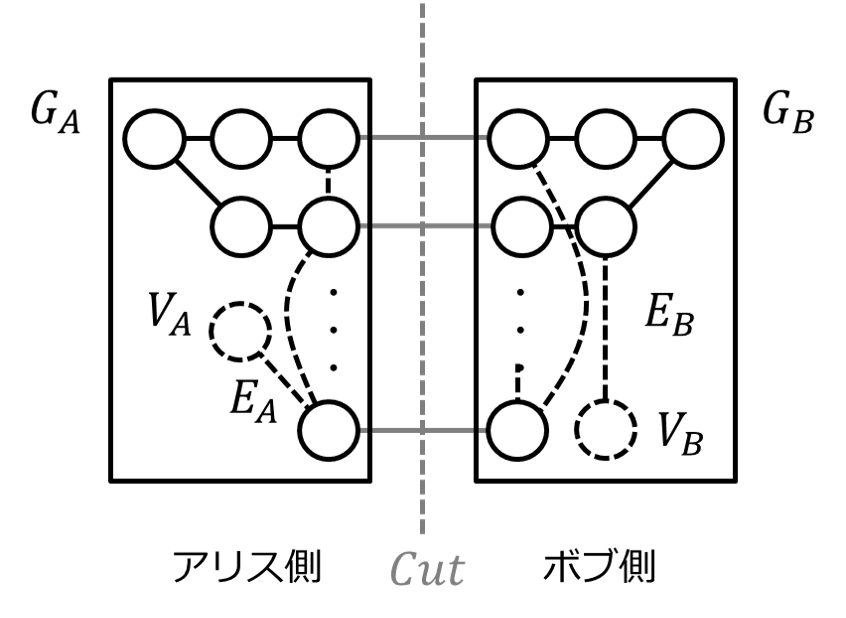
\includegraphics[width=120mm]{Gxy.png}
\end{center}
\caption{$G^{x, y} = (V', E')$}
\label{Gxy}
\end{figure}

アリスとボブは,入力グラフ上に特性$P$があるかを判定する分散アルゴリズムをシミュレートできる.
アリスは$G_{A}$に含まれる頂点を,ボブは$G_{B}$に含まれる頂点をシミュレートする.
2者間通信複雑性モデルでのシミュレートは,次のように実行される.$G_{A}$中の辺で送信されるメッセージ,あるいは
$G_{B}$中の辺で送信されるメッセージは,アリスとボブがそれぞれお互いと通信せずにシミュレートできる.カット辺$C$を通じて
送信されるメッセージに対しては,お互い情報を交換する必要がある.{\CONGEST}モデルにおいてグラフ上に特性$P$が
あるかどうかを$r$ラウンドで判定するアルゴリズム$\mathcal{A}$が存在したとすると,アリスとボブは特性$P$の判定のために
$O(r \cdot |C| \cdot \log n)$ビット通信したことになる.これは,各ラウンドで,アルゴリズムが各辺で$O(\log n)$ビットの通信を
行っているからである.このグラフにおいてアルゴリズム$\mathcal{A}$を実行すると同時に2者間交叉判定問題も解けていることになる.
例えばアルゴリズムを実行した結果,入力グラフに特性$P$があると判定されれば$DISJ_{k} (x, y)=1$であると分かるからである.
交叉判定問題の通信複雑性よりアリスとボブは少なくとも$\Omega (k)$ビットは通信しているはずである.
したがって,$CONGEST$モデルにおいてと特性$P$があるかどうかを判定する任意のアルゴリズムに対して
$r = \Omega (k / |C| \cdot \log n)$ラウンドの下界を得ることができる.カット辺の大きさが小さくなるほど下界が強くなる.
\newpage

\chapter{1-MIS検証問題の$O(1)$ラウンドアルゴリズム}
この章では,1-MIS検証問題を$O(1)$ラウンドで解くアルゴリズムついて述べる. \\
{\CONGEST}モデルにおいて,入力としてグラフ$G$と独立集合$I$が与えられたとき,
1-MIS検証問題を解くために次のようなアルゴリズム$\mathcal{A}$を実行する.
\begin{enumerate}
\item 各頂点$v \in I$は,自分のIDである$v$.idを隣接頂点全員に送信する.
\item 各頂点$u \notin I$のうち,2種類以上のIDをもらった頂点は0を返し,アルゴリズムから離脱する.
\item 離脱しなかった頂点$u \notin I$のうち,1種類だけのID($v$.idとする)を受信した頂点は
離脱していない全隣接頂点へ$v$.idを送信する.
頂点$u \notin I$は,自身が持つ$v$.idと違う$v$.idが書かれたメッセージは無視し,
自身が持つ$v$.idと同じ$v$.idが書かれたメッセージの数を記憶し,それを$u.a$とする.
\item 各頂点$v \in I$は,自身と同じ$v$.idを返信してきた頂点の集合($v.X$とする)を記憶する.
その後サイズ$|v.X|$を$v.X$中の頂点に送信し,0を返す.
\item メッセージを受け取った$v.X$中の頂点$u$は,送られたサイズ$|v.X| - 1$と$u.a$を比較する.
$|v.X | - 1 = u.a$であれば頂点$u$は$0$を返し,そうでなければ$u$は1を返す.
\end{enumerate}

アルゴリズム$\mathcal{A}$の各ステップは明らかに$O(1)$ラウンドで{\CONGEST}モデルで実装できる.
アルゴリズム$\mathcal{A}$について,以下の補題が成り立つ.
\begin{lemma}
アルゴリズム$\mathcal{A}$は1-MIS検証問題を解くことができる.
\end{lemma}
\begin{prf*}
アルゴリズム$\mathcal{A}$は与えられた入力に対して誤った答えを返すとする.
このとき以下の2つのうち,どちらかが成り立つ. \\
1.与えられた独立集合が1-MISであり,アルゴリズム$\mathcal{A}$が1-MISでないと返す. \\
2.与えられた独立集合が1-MISでなく,アルゴリズム$\mathcal{A}$が1-MISであると返す. \\

アルゴリズム$\mathcal{A}$の5番目のステップで$|v.X| - 1$と$a$を比較して,
$v.X$に含まれる任意の頂点$u$で$|v.X| - 1 = u.a$が成り立つとき$v.X$の頂点はクリークを形成している.
これは$v.X$に含まれる頂点$u \notin I$で等号が成立するのは$u$が$v.X \backslash \{u\}$に含まれる
全ての頂点と隣接している場合のみだからである.

1.の場合,アルゴリズム$\mathcal{A}$が1-MISでないと返したということは,ある$v.X$について
その中の頂点$u \notin I$が1を返したということである.
この場合,$v.X$に含まれる頂点で$u$に隣接していない頂点$w$が存在するはずである.
また$u$と$w$に隣接する$I$内の頂点は$v$のみである.従って$v$を$I$から取り除いて
$u$と$w$を$I$に追加することで独立集合を維持しつつサイズを大きくすることができるため
与えられた独立集合は1-MISではないが,これは仮定に矛盾する. 

2.の場合,アルゴリズム$\mathcal{A}$が1-MISであると返したということは,全ての$v.X$について
その中の頂点$u \notin I$が0を返したということである.この場合,全ての$v.X$がクリークを形成している.
従って,$v.X$の中には独立集合に追加できる可能性のある頂点は存在しない.また,2番目のステップで
離脱した頂点も独立集合点に含まれている1頂点を取り除いただけ追加できる可能性はない.
よって,独立集合を維持しつつサイズを大きくするために追加できる頂点は存在しないため
与えられた独立集合は1-MISであるが,これは仮定に矛盾する. 

以上より,アルゴリズム$\mathcal{A}$は与えられた入力に対して正しい答えを返すことができるため,
1-MIS検証問題を解くことができる.
\end{prf*}
\newpage

\chapter{$k$-MIS検証問題の下界}
この章では,$k$-MIS検証問題の下界についての議論を行う.
4.1節では,2-MIS検証問題の下界についての定理とその証明を述べる.
4.2節では,3-MIS検証問題の下界についての定理とその証明を述べる.
4.3節では,$k$-MIS検証問題($k = 4l + 5, l \geq 1$)の下界についての定理とその証明を述べる.

\section{2-MIS検証問題の下界}

この節では2-MIS検証問題の下界についての議論を行う.具体的には,次の定理を証明する.
\begin{theorem}
{\CONGEST}モデルにおいて,2-MIS検証問題を解く全てのアルゴリズムは$\tilde{\Omega} (\sqrt{n})$の
通信ラウンド数を必要とする.
\end{theorem}
\begin{prf*}
まず初めにアリスとボブが構築するグラフ$G = (V, E)$を図 \ref{2_G}に示す. 

\begin{figure}[ht]
\begin{center}
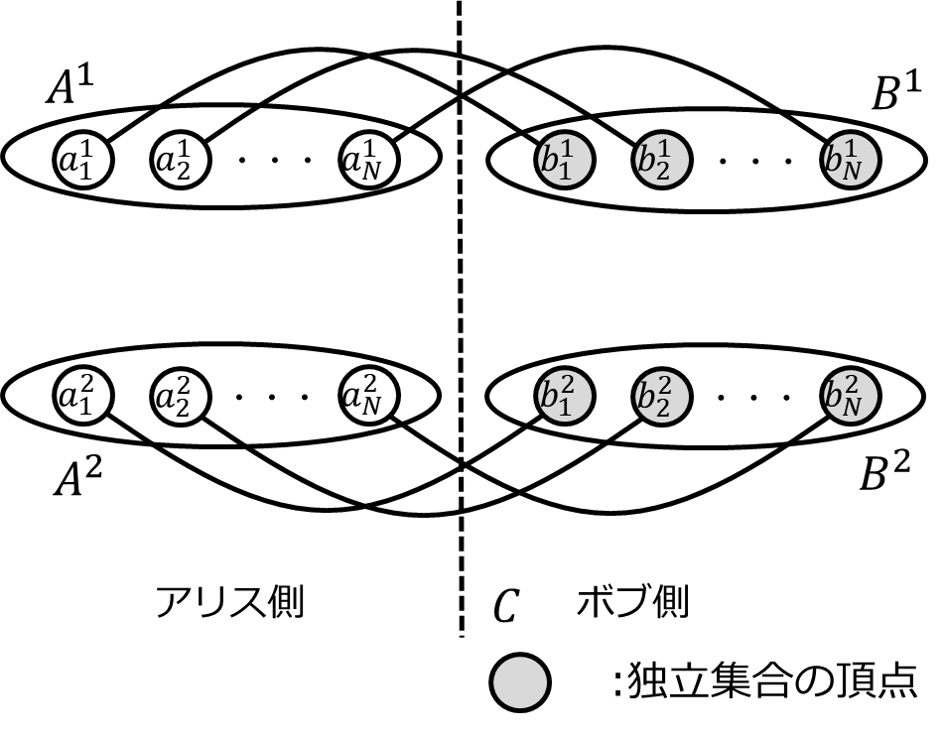
\includegraphics[width=120mm]{2_G.png}
\end{center}
\caption{$G = (V, E)$}
\label{2_G}
\end{figure}

図中の頂点のうち灰色のものは独立集合に含まれる頂点とする.図中の辺を定式化すると以下のようになる.
\Izumi{まず最初に,帰着に使うグラフの形式的な定義を書く(頂点集合,辺集合をちゃんと形式的に定義する).
手続き的に少しづつ頂点集合や辺集合を導入していって構成する必要はない,「XXXはクリークを成している」と
するだけで辺集合を説明するのもよくないので避ける(形式的な定義を示したのち「すなわち,XXXはクリークを構成している」と補足的に説明するのが良い.図4.1は中途半端なので,なくてもいいのでは?}
%図中の頂点のうち,灰色のものは独立集合に含まれる頂点とする.図中で省略されている辺と$K_{W(y)}$の構造は次のとおりである.
\begin{itemize}
\item $\forall i((a_{i}^{1}, b_{i}^{1}), (a_{i}^{2}, b_{i}^{2})) \in E$
\end{itemize}


このグラフが「$G$中に与えられている独立集合が,$DISJ_{N \times N} (x, y) = 1$のときのみ2-MISでない」という特性$P_{2}$を持つように,
$G_{A}$に構造$H_{A}$,$G_{B}$に構造$H_{B}$を追加する.
(なお,$DISJ_{N \times N} (x, y) :=\bigvee_{i = 1}^{N} \bigvee_{j = 1}^{N} x_{i, j} \land y_{i, j}$で定義される.)
$H_{A}$と$H_{B}$の中身は以下のとおりである.

\newpage
\begin{itemize}
\item $H_{A}$: $(a_{i}^{1}, a_{j}^{2}) \in E_{A} \Leftrightarrow x_{i, j} = 0$
\item $H_{B}$: $W(y)$頂点のクリーク$K_{W(y)}$($W(y)$は0/1のデータ列$y$中に含まれる1の個数を表す.)
$K_{W(y)}$中の頂点$c_{i, j} \in V_{B}$は$y_{i, j} = 1$であるような$(i, j)$でインデックスづけされるものとする. \\
このとき,$(c_{i, j}, b_{i}^{1}) \in E_{B}$ かつ $(c_{i, j}, b_{j}^{2}) \in E_{B}$
\end{itemize}

$G = (V, E)$に辺と頂点を追加したグラフ$G^{x, y} = (V', E')$を図 \ref{2_G(x,y)}に示す.

\begin{figure}[ht]
\begin{center}
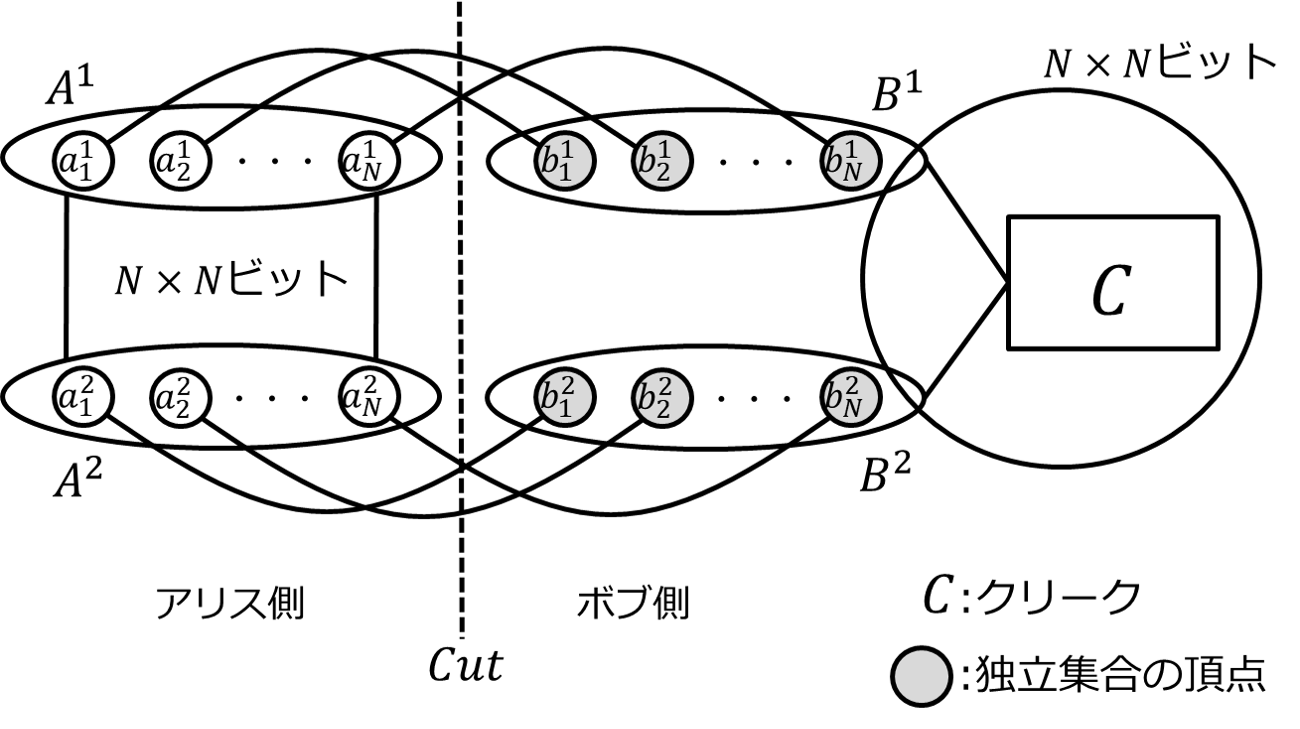
\includegraphics[width=120mm]{2_Gxy.png}
\end{center}
\caption{$G^{x, y} = (V', E')$}
\label{2_G(x,y)}
\end{figure}

このグラフ$G^{x, y} = (V', E')$が上記の特性$P_{2}$を満たしていることを示すために,次の2点を確認する. \\
(i)$DISJ_{N \times N} (x, y) = 1$のとき,グラフに与えられている独立集合が2-MISでない: \\
$x_{i, j} = y_{i, j} =1$とすると,$b_{i}^{1}$と$b_{j}^{2}$の2点を取り除いて$a_{i}^{1}$, $a_{j}^{2}$, $c_{i, j}$の
3点を追加できることから確認できる. \\
(ii)$DISJ_{N \times N} (x, y) = 0$のとき,グラフに与えられている独立集合が2-MISである: \\ 
グラフに与えられている独立集合が2-MISでないと仮定する.このとき,ある2点を取り除くことで独立集合に追加できる3点が存在する.
2点の取り除き方は(1)$b_{i}^{1}$と$b_{j}^{1}(i \neq j)$, (2)$b_{i}^{2}$と$b_{j}^{2}(i \neq j)$, (3)$b_{i}^{1}$と$b_{j}^{2}$が考えられる.
(1)では$a_{i}^{1}$と$a_{j}^{1}$の2点しか追加できる可能性がなく,(2)では$a_{i}^{2}$と$a_{j}^{2}$の2点しか追加できる可能性がない.
(3)において,$b_{i}^{1}$を取り除いて$a_{i}^{1}$を追加し,$b_{j}^{2}$を取り除いて$a_{j}^{2}$を追加し,さらに$c_{i, j}$を追加することを考える.
$a_{i}^{1}$と$a_{j}^{2}$が両方とも追加できるのは$x_{i, j} = 1$のときのみであり,$c_{i, j}$が追加できる($c_{i, j}$が存在する)のは
$y_{i, j} = 1$のときのみであるが,これは$DISJ_{N \times N} (x, y) = 0$に矛盾する.したがってグラフに与えられている独立集合から2点取り除いて
3点追加することはできないため,この独立集合は2-MISである.

今回,$N \times N$ビットの交叉判定インスタンスをグラフに埋め込んでおり,カット辺のサイズ$|C| = 2N$であることが分かる.
{\CONGEST}モデルにおいてグラフ上に与えられた独立集合が2-MISであるかどうかを$r$ラウンドで判定する
アルゴリズム$\mathcal{A}$が存在したとすると,アリスとボブは$O(r \cdot |C| \cdot \log n)$ビット通信したことになる.
このグラフにおいてアルゴリズム$\mathcal{A}$を実行すると同時に2者間交叉判定問題も解けていることになるので,
交叉判定問題の通信複雑性よりアリスとボブは少なくとも$\Omega (N \times N)$ビットは通信しているはずである.
よって,$r = \Omega (N / 2\log n) = \tilde{\Omega}(N)$ラウンドの下界を得ることができる.図\ref{2_G(x,y)}から分かる通り,
$A^{1}, A^{2}, B^{1}, B^{2}$はそれぞれ$N$頂点で構成されており,$K_{W(y)}$の頂点数は$O(N^{2})$であるため,
グラフ全体の頂点数$n$は$n = O(N + N^{2})$である.したがって$N = \Omega(\sqrt{n})$になるため,
$\tilde{\Omega}(\sqrt{n})$ラウンドの下界を得ることができる.
\end{prf*}
\newpage

\section{3-MIS検証問題の下界}
この節では3-MIS検証問題の下界についての議論を行う.具体的には,次の定理を証明する.
\begin{theorem}
{\CONGEST}モデルにおいて,3-MIS検証問題を解く全てのアルゴリズムは$\tilde{\Omega} (n)$の通信ラウンド数を必要とする.
\end{theorem}

\begin{prf*}
まず初めにアリスとボブが構築するグラフ$G = (V, E)$を図 \ref{3_G}に示す.

\begin{figure}[ht]
\begin{center}
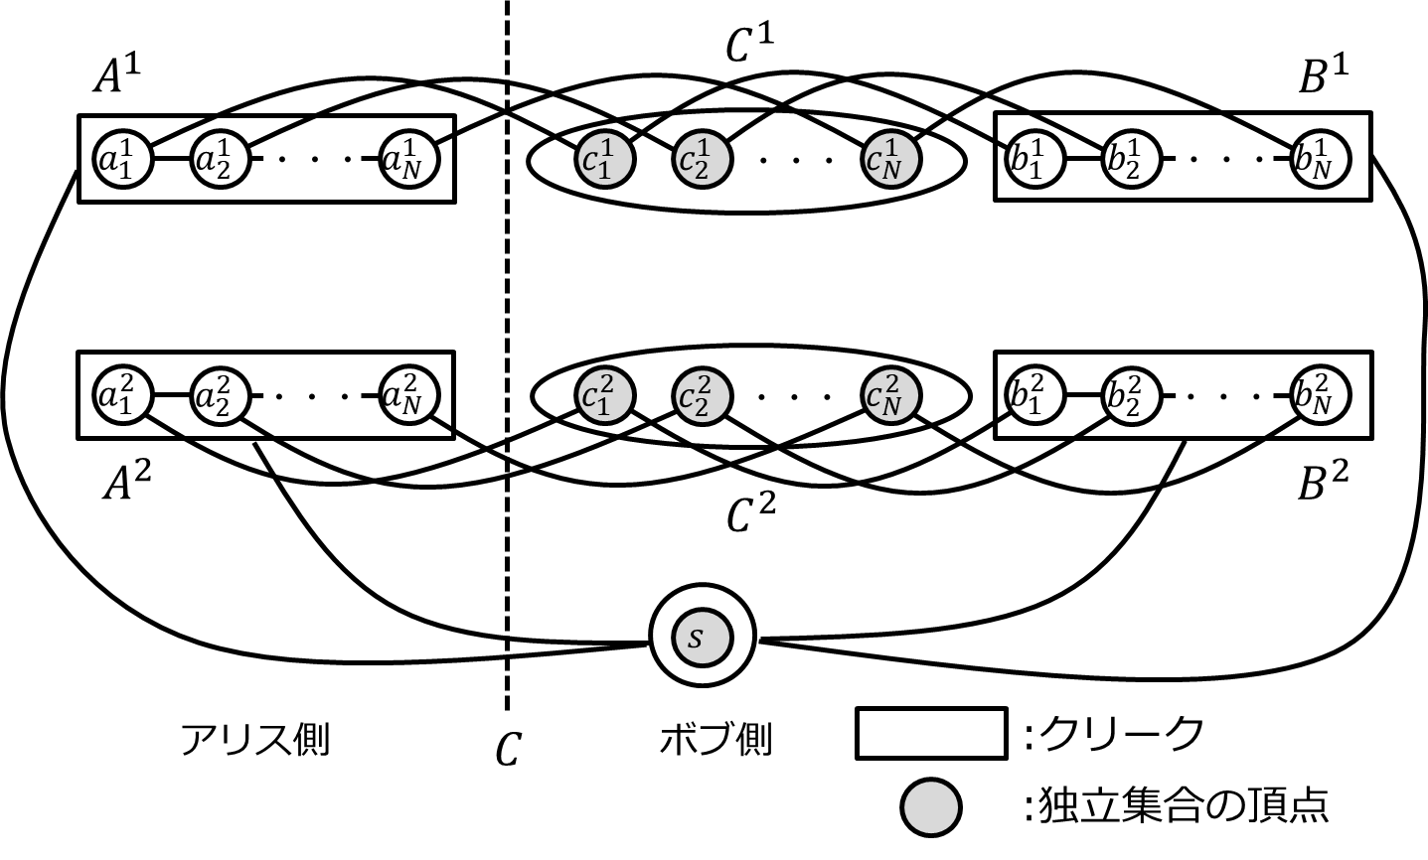
\includegraphics[width=120mm]{3_G.png}
\end{center}
\caption{$G = (V, E)$}
\label{3_G}
\end{figure}

図中の頂点のうち灰色のものは独立集合に含まれる頂点とする.また,四角で囲まれている部分はクリークを表す.
図中の辺を定式化すると以下のようになる.
\Izumi{こちらも記述の仕方は2-MISの時と同様に}
\begin{itemize}
\item $A^{1}, A^{2}, B^{1}, B^{2}$は$N$頂点のクリーク$K_{N}$
\item $\forall i((a_{i}^{1}, c_{i}^{1}), (a_{i}^{2}, c_{i}^{2}), (b_{i}^{1}, c_{i}^{1}), (b_{i}^{2}, c_{i}^{2})) \in E$
\item $\forall i((a_{i}^{1}, s), (a_{i}^{2}, s), (b_{i}^{1}, s), (b_{i}^{2}, s)) \in E$
\end{itemize}

このグラフが「$G$中に与えられている独立集合が,$DISJ_{N \times N} (x, y) = 1$のときのみ3-MISでない」という特性$P_{3}$を持つように,
$G_{A}$に構造$H_{A}$,$G_{B}$に構造$H_{B}$を追加する.$H_{A}$と$H_{B}$の中身は以下のとおりである.
\newpage
\begin{itemize}
\item $H_{A}$: $(a_{i}^{1}, a_{j}^{2}) \in E_{A} \Leftrightarrow x_{i, j} = 0$
\item $H_{B}$: $(b_{i}^{1}, b_{j}^{2}) \in E_{B} \Leftrightarrow y_{i, j} = 0$
\end{itemize}

$G = (V, E)$に辺を追加したグラフ$G^{x, y} = (V, E')$を図 \ref{3_G(x,y)}に示す.

\begin{figure}[ht]
\begin{center}
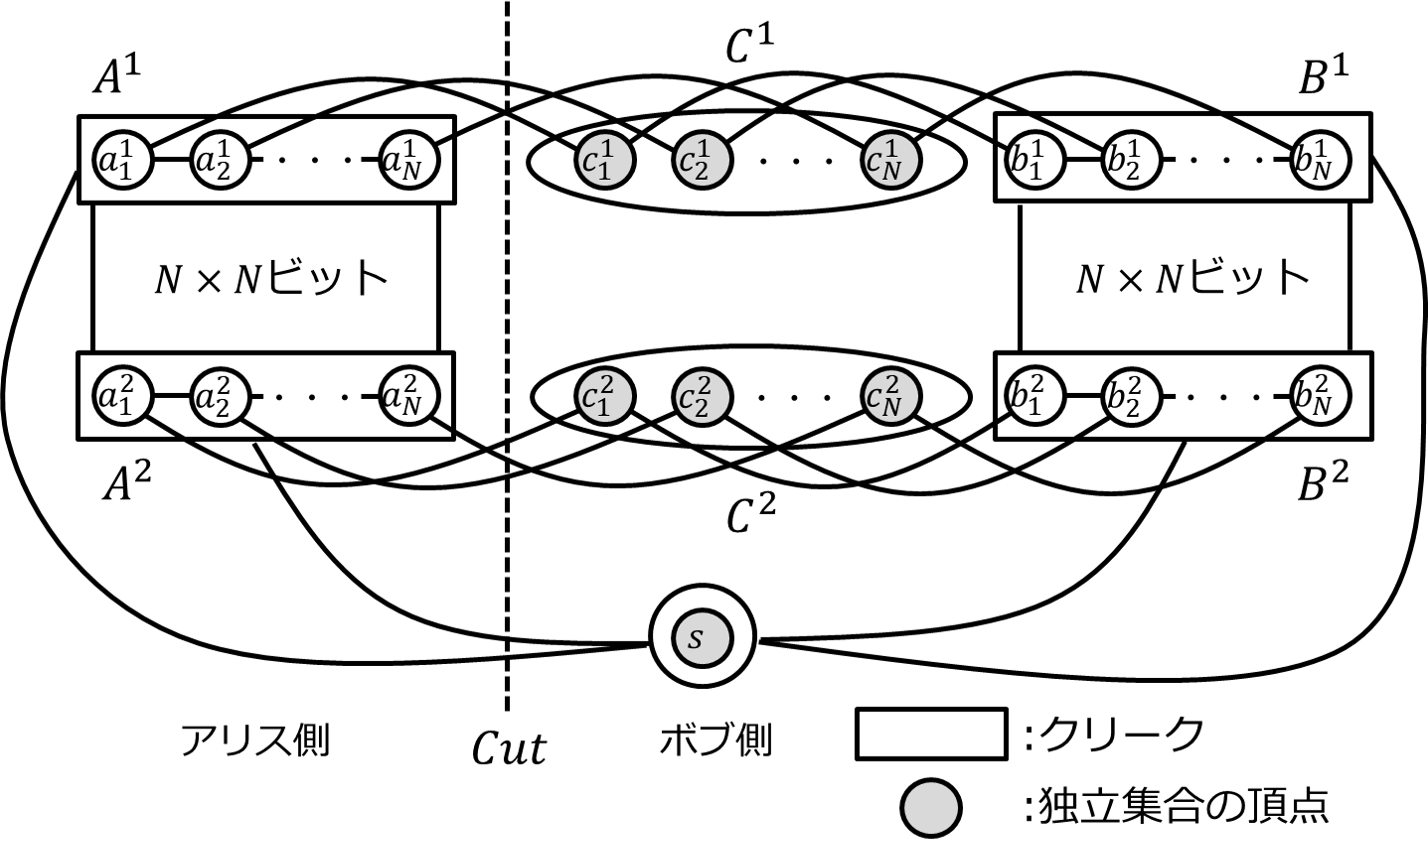
\includegraphics[width=120mm]{3_Gxy.png}
\end{center}
\caption{$G^{x, y} = (V, E')$}
\label{3_G(x,y)}
\end{figure}

このグラフ$G^{x, y} = (V, E')$が上記の特性$P_{3}$を満たしていることを示すために,次の2点を確認する. \\
(i)$DISJ_{N \times N} (x, y) = 1$のとき,グラフに与えられている独立集合が3-MISでない: \\
$x_{i, j} = y_{i, j} =1$とすると,$s$と$c_{i}^{1}$と$c_{j}^{2}$の3点を取り除いて$a_{i}^{1}$, $b_{i}^{1}$, $a_{j}^{2}$, $c_{j}^{2}$の
4点を追加できることから確認できる。 \\
(ii)$DISJ_{N \times N} (x, y) = 0$のとき,グラフに与えられている独立集合が3-MISである: \\ 
グラフに与えられている独立集合が3-MISでないと仮定する.このとき,ある3点を取り除くことで独立集合に追加できる4点が存在するが,
$A^{1}, A^{2}, B^{1}, B^{2}$がそれぞれクリークであるため,4点を追加するためにはそれぞれから1点を選ぶ必要がある.
$c_{i}^{1}$を取り除いて$a_{i}^{1}$と$b_{i}^{1}$を追加し,$c_{j}^{2}$を取り除いて,$a_{j}^{2}$と$b_{j}^{2}$を独立集合に追加したとする.
$a_{i}^{1}$と$a_{j}^{2}$が両方とも追加できるのは$x_{i, j} = 1$のときのみであり,$b_{i}^{1}$と$b_{j}^{2}$が両方とも追加できるのは
$y_{i, j} = 1$のときのみであるが,これは$DISJ_{N \times N} (x, y) = 0$に矛盾する。したがってグラフに与えられている独立集合から3点取り除いて
4点追加することはできないため,この独立集合は3-MISである.

今回,$N \times N$ビットの交叉判定インスタンスをグラフに埋め込んでおり,カット辺のサイズ$|C| = 4N$であることが分かる.
{\CONGEST}モデルにおいてグラフ上に与えられた独立集合が3-MISであるかどうかを$r$ラウンドで判定する
アルゴリズム$\mathcal{A}$が存在したとすると,アリスとボブは$O(r \cdot |C| \cdot \log n)$ビット通信したことになる.
このグラフにおいてアルゴリズム$\mathcal{A}$を実行すると同時に2者間交叉判定問題も解けていることになるので,
交叉判定問題の通信複雑性よりアリスとボブは少なくとも$\Omega (N \times N)$ビットは通信しているはずである,
よって,$r = \Omega (N / 4\log n) = \tilde{\Omega}(N)$ラウンドの下界を得ることができる.図\ref{3_G(x,y)}から分かる通り,
$A^{1}, A^{2}, B^{1}, B^{2}, C^{1}, C^{2}$はそれぞれ$N$頂点で構成されているため,グラフ全体の頂点数$n$は$n = O(N)$である.
したがって$N = \Omega(n)$になるため,$\tilde{\Omega}(n)$ラウンドの下界を得ることができる.
\end{prf*}
\newpage

\section{$k$-MIS検証問題の下界}
このセクションではk-MIS検証問題の下界についての議論を行う.具体的には,次の定理を証明する.
\begin{theorem}
{\CONGEST}モデルにおいて,任意の$l \geq 1$に対して$k = 4l + 5$としたとき$k$-MIS検証問題を解く全てのアルゴリズムは
$\Omega\left(n^{2 - \frac{1}{l+1}}/l\right)$の通信ラウンド数を必要とする.
\end{theorem}

\begin{prf*}
以下をを定義する.
\begin{definition}
証明の簡略化のために$N$の$l + 1$乗根は整数であると仮定する.このとき$M = \sqrt[l + 1]{N}$とする.
また,自然数$i, j, h$が与えられたとき,$\alpha_{i, h}(j)$を$j$を$i$進数で表したときの$h$桁目の値と定義する.
\end{definition}
まず初めにアリスとボブが構築するグラフ$G = (V, E)$を図 \ref{k_G}に示す.

\begin{figure}[ht]
\begin{center}
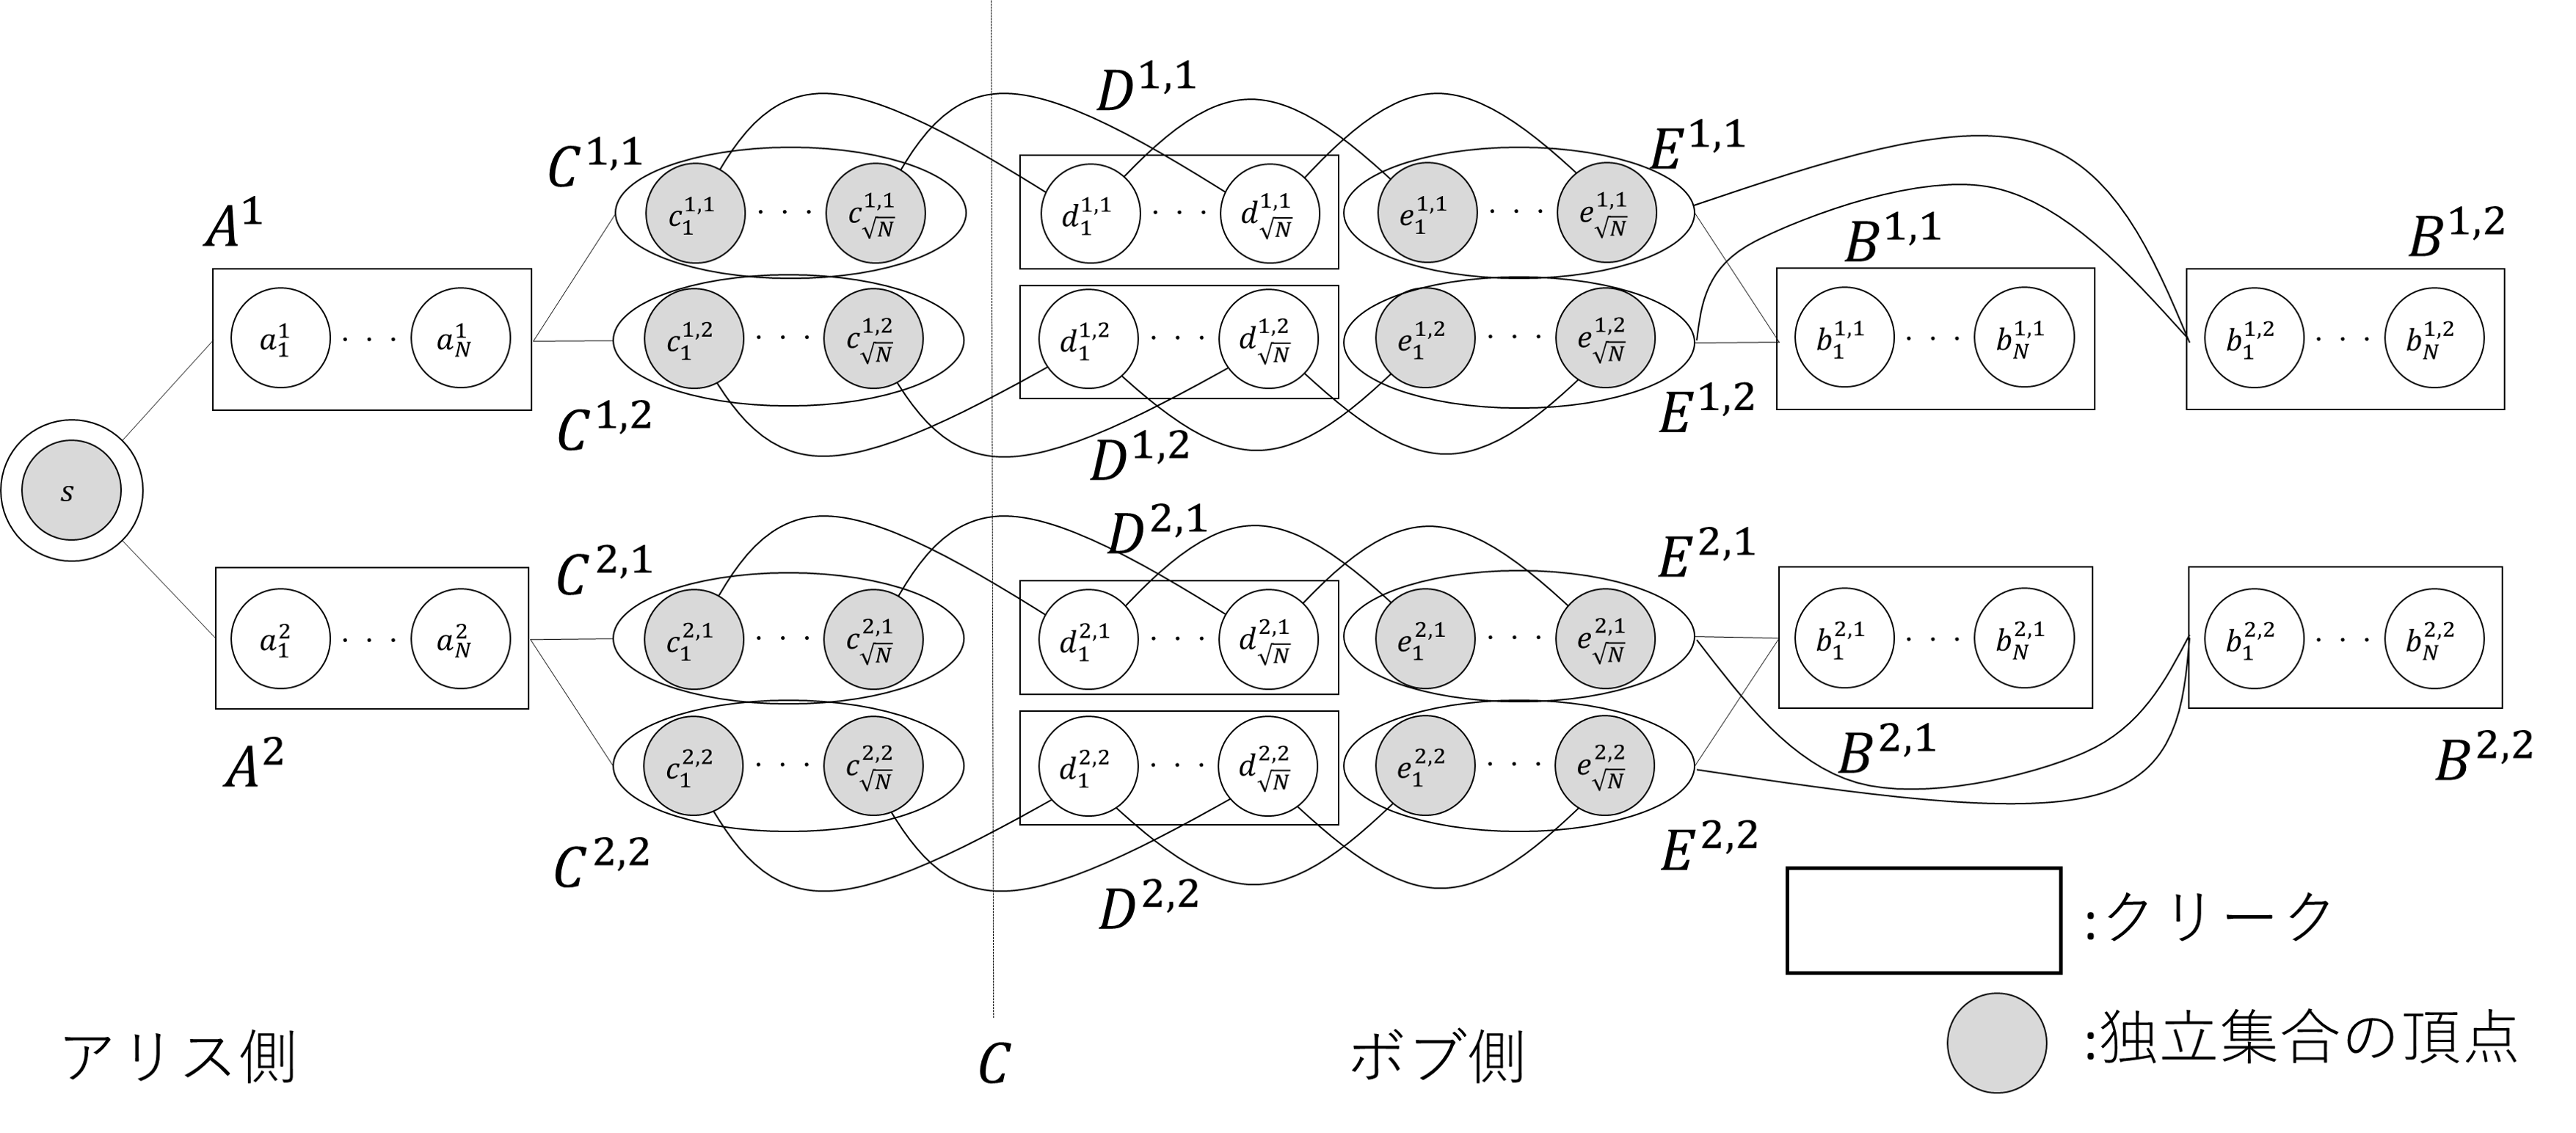
\includegraphics[width=120mm]{k_G.png}
\end{center}
\caption{$G = (V, E)$}
\label{k_G}
\end{figure}

図中の頂点のうち灰色のものは独立集合に含まれる頂点とする.また,四角で囲まれている部分はクリークを表す.
図中の辺を定式化すると以下のようになる.
\begin{itemize}
\item $A^{1}=\{a^{1}_{1},\dots,a^{1}_{N}$\}と
$A^{2}=\{a^{2}_{1},\dots,a^{2}_{N}\}$は$N$頂点のクリーク
\item 任意の$1\leq i \leq l+1$に対して$B^{1}_{i}=\{b^{1,i}_{1},\dots,b^{1,i}_{N}\}$と
$B^{2}_{i}=\{b^{2,i}_{1},\dots,b^{2,i}_{N}\}$は$N$頂点のクリーク
\item 任意の$1\leq i \leq l+1$に対して$D^{1}_{i}=\{d^{1,i}_{1},\dots,d^{1,i}_{M}\}$と
$D^{2}_{i}=\{d^{2,i}_{1},\dots,d^{2,i}_{M}\}$は$M$頂点のクリーク
\item $\forall i((a_{i}^{1}, s), (a_{i}^{2}, s)) \in E$
\item 任意の$1\leq i \leq N$と$1\leq j \leq l+1$に対して$\left(a^{1}_{i},c^{1,j}_{\alpha_{M,j}(i-1)+1}\right)$と$\left(a^{2}_{i},c^{2,j}_{\alpha_{M,j}(i-1)+1}\right)$が$E$に含まれる
\item 任意の$1\leq i \leq N$,$1\leq j \leq l+1$と$1\leq h \leq l+1$に対して$\left(b^{1,h}_{i},e^{1,j}_{\alpha_{M,j}(i-1)+1}\right)$と$\left(b^{2,h}_{i},e^{2,j}_{\alpha_{M,j}(i-1)+1}\right)$が$E$に含まれる
\item 任意の$1\leq i \leq M$と$1\leq j \leq l+1$に対して$(c_{i}^{1, j}, d_{i}^{1, j})$と$(e_{i}^{1, j}, d_{i}^{1, j})$が$E$に含まれる
\item 任意の$1\leq i \leq M$と$1\leq j \leq l+1$に対して$(c_{i}^{2, j}, d_{i}^{2, j})$と$(e_{i}^{2, j}, d_{i}^{2, j})$が$E$に含まれる
\end{itemize}

このグラフが「$G$中に与えられている独立集合が,$DISJ_{N \times N} (x, y) = 1$のときのみ
$k$-MISでない」という特性($P_{k}$)を持つように,
$G_{A}$に構造$H_{A}$,$G_{B}$に構造$H_{B}$を追加する.$H_{A}$と$H_{B}$の中身は以下のとおりである.

\begin{itemize}
\item $H_{A}$: $E_{A}=\{(a^{1}_{i},a^{2}_{j}) \mid x_{i,j}=0, 1 \leq i \leq N, 1 \leq j \leq N\}$
\item $H_{A}$: $E_{B}=\{(a^{1,h}_{i},a^{2,h}_{j}) \mid x_{i,j}=0, 1 \leq i \leq N, 1 \leq j \leq N, 1 \leq h \leq l+1\}$
\end{itemize}

$G = (V, E)$に辺を追加したグラフ$G^{x, y} = (V, E')$を図 \ref{k_Gxy}に示す.

\begin{figure}[ht]
\begin{center}
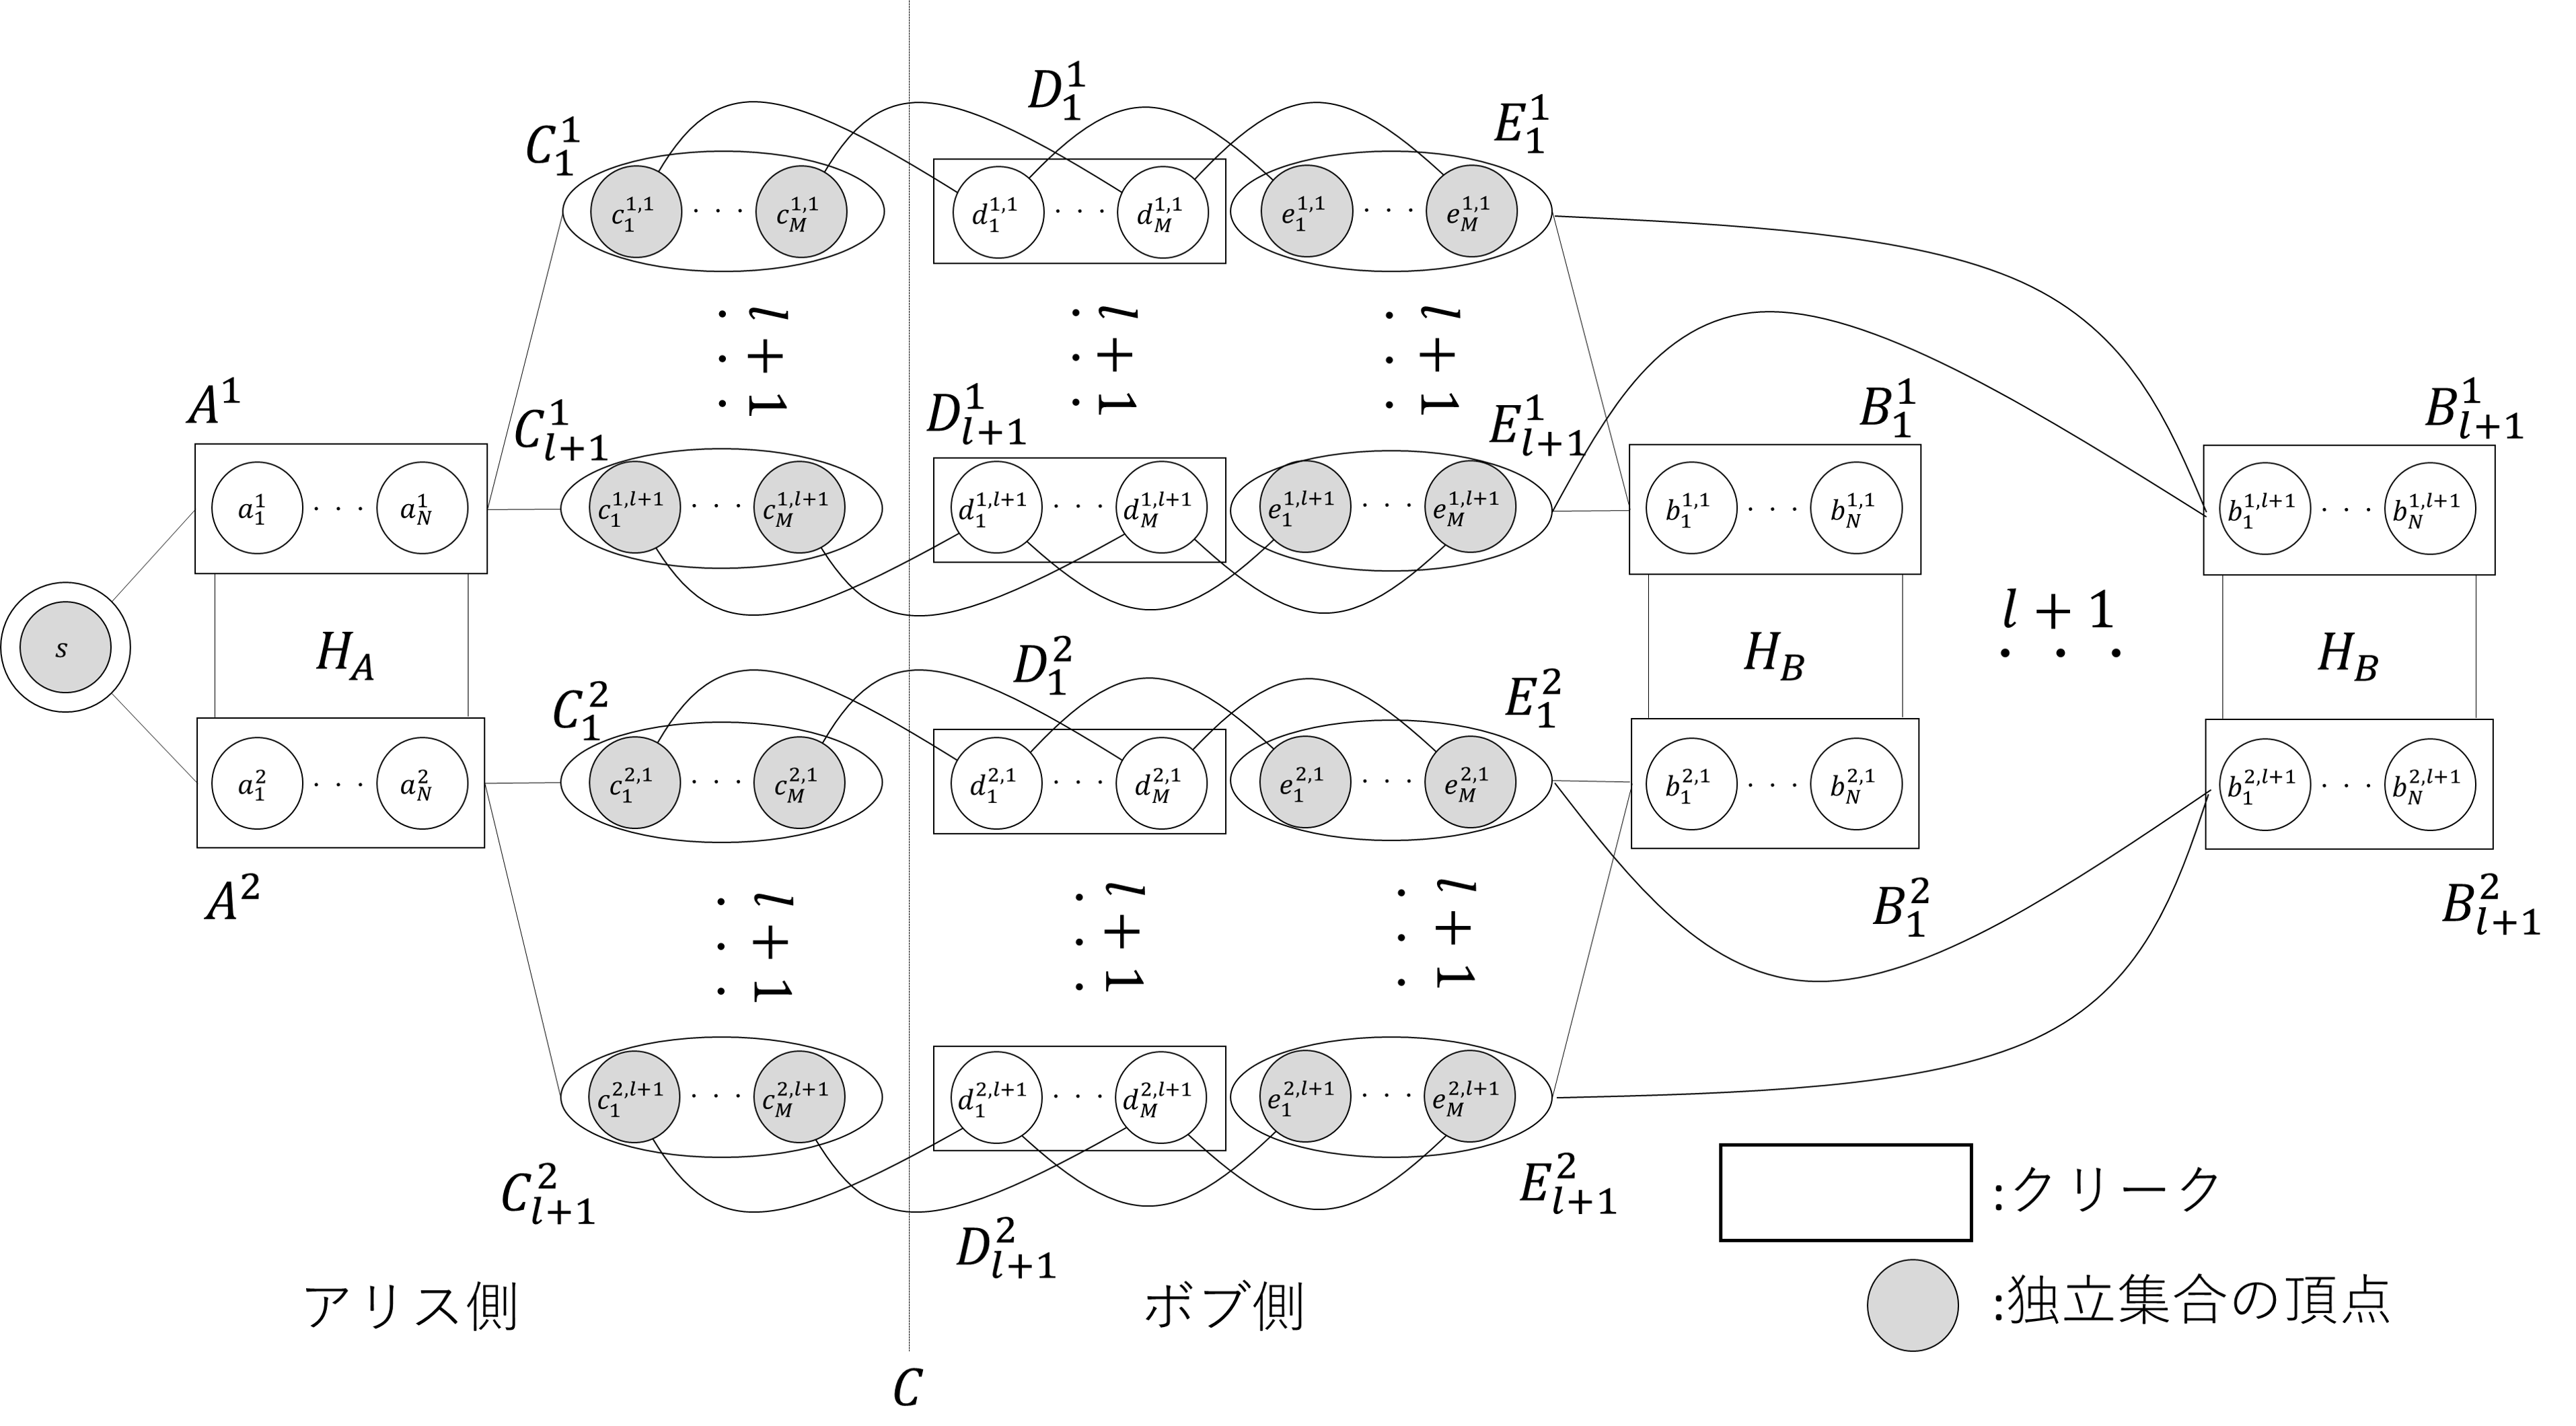
\includegraphics[width=120mm]{k_Gxy.png}
\end{center}
\caption{$G^{x, y} = (V, E')$}
\label{k_Gxy}
\end{figure}

このグラフ$G^{x, y} = (V, E')$が上記の特性($P_{k}$)を満たしていることを示すために,次の2点を確認する. \\
(i)$DISJ_{N \times N} (x, y) = 1$のとき,グラフに与えられている独立集合が$k$-MISでない: \\
$x_{i,j}=y_{i,j}=1$であると仮定する.このとき,
\begin{dmath*}
I'=\{s\} \cup \bigcup_{1\leq h \leq l+1}c^{1,h}_{\alpha_{M,h}(i-1)+1} \cup 
\bigcup_{1\leq h \leq l+1}c^{2,h}_{\alpha_{M,h}(j-1)+1} \cup 
\bigcup_{1\leq h \leq l+1}e^{1,h}_{\alpha_{M,h}(i-1)+1} \cup 
\bigcup_{1\leq h \leq l+1}e^{2,h}_{\alpha_{M,h}(j-1)+1}
\end{dmath*}
\begin{dmath*}
S=\{a^{1}_{i} \cup a^{2}_{j}\} \cup 
\bigcup_{1\leq h \leq l+1}b^{1,h}_{j} \cup 
\bigcup_{1\leq h \leq l+1}b^{2,h}_{j} \cup 
\bigcup_{1\leq h \leq l+1}d^{1,h}_{\alpha_{M,h}(i-1)+1} \cup  
\bigcup_{1\leq h \leq l+1}d^{2,h}_{\alpha_{M,h}(j-1)+1}
\end{dmath*}
とすると
$I \backslash I' \cup S$は独立集合になる.ここで$|I'|=4l+5$で$|S|=4l+6$であることから,
$k=4l+5$に対して$I$は$k$-MISでないことが確認できる. \\
(ii)$DISJ_{N \times N} (x, y) = 0$のとき,グラフに与えられている独立集合が$k$-MISである: \\ 
グラフに与えられている独立集合が$k$-MISでないと仮定する.このとき,$I'\subseteq I$をサイズ$k$以下の独立集合,
$S\subseteq V\backslash I$を$(I \backslash I') \cup S$が独立集合になるサイズ$|I'|+1$以上の頂点集合とする.
また,$(A^{1}\cup A^{2}) \cap S$を満たす頂点の数を$num(A)$,
$\bigcup_{1\leq i \leq l+1}(B_{i}^{1} \cup B_{i}^{2}) \cap S$を満たす頂点の数を$num(B)$,
$\left(\bigcup_{1\leq i \leq l+1}C_{i}^{1} \cup \bigcup_{1\leq i \leq l+1}C_{i}^{2}\right) \cap S$を満たす頂点の数を$num(C)$,
$\left(\bigcup_{1\leq i \leq l+1}D_{i}^{1} \cup \bigcup_{1\leq i \leq l+1}D_{i}^{2}\right) \cap S$を満たす頂点の数を$num(D)$,\\
$\left(\bigcup_{1\leq i \leq l+1}E_{i}^{1} \cup \bigcup_{1\leq i \leq l+1}E_{i}^{2}\right) \cap S$を満たす頂点の数を$num(E)$とする.
 任意の$1\leq i \leq M$と$1\leq j \leq l+1$に対して$d^{1,j}_{i}$を独立集合に追加するには
 $c^{1,j}_{i}$と$e^{1,j}_{i}$を独立集合から取り除く必要がある.
また,任意の$1\leq i \leq M$と$1\leq j \leq l+1$に対して$d^{2,j}_{i}$を独立集合に追加するには
$c^{2,j}_{i}$と$e^{2,j}_{i}$を独立集合から取り除く必要がある.
従って,$num(D)$の値は$num(C)$によって上から抑えられる.また,$num(D)$の値は$num(E)$によっても上から抑えられる.
任意の$1\leq i \leq N$と$1\leq j \leq l+1$に対して,$b^{1,j}_{i}$を独立集合に追加するには,
$\bigcup_{1\leq h \leq l+1} e^{1,h}_{\alpha_{M,h}(i-1)+1}$を独立集合から取り除く必要がある.
従って,任意の$1\leq i \leq l+1$に対して$B^{1}_{i}$に含まれる頂点を独立集合に追加するには
$\bigcup_{1\leq j \leq l+1}E^{1}_{j}$に含まれる頂点を少なくとも$l+1$個独立集合から取り除く必要がある.
同様に任意の$1\leq i \leq N$と$1\leq j \leq l+1$に対して,$b^{2,j}_{i}$を独立集合に追加するには,
$\bigcup_{1\leq h \leq l+1} e^{1,h}_{\alpha_{M,h}(i-1)+1}$を独立集合から取り除く必要がある.
従って,任意の$1\leq i \leq l+1$に対して$B^{2}_{i}$に含まれる頂点を独立集合に追加するには
$\bigcup_{1\leq j \leq l+1}E^{2}_{j}$に含まれる頂点を少なくとも$l+1$個独立集合から取り除く必要がある.
任意の$1\leq i \leq 2$と$1\leq j \leq l+1$に対して,$B^{i}_{j}$はクリークであるので,
$B^{i}_{j}$に含まれる頂点は高々1つしか独立集合に加えることができない.
従って$\bigcup_{1\leq i \leq l+1}B^{1}_{i}$から独立集合に加えられる頂点の数は高々$l+1$個であり,
$\bigcup_{1\leq i \leq l+1}B^{2}_{i}$から独立集合に加えられる頂点の数は高々$l+1$個であるので,
$num(B)$の値は$num(E)$の値によって上から抑えられる.
従って$|S|\geq |I'|+1$を満たすには$(num(A) \geq 1$である必要があるが,
$A^{1}$と$A^{2}$はそれぞれクリークあるため$num(A) = 1$もしくは$num(A) = 2$である.\\
はじめに$num(A)=1$の場合を考える.
このとき,$A^{1} \cup A^{2}$に含まれる頂点を独立集合に追加するには頂点$s$を
独立集合から取り除かなければならない.
従って$|I'|=1+num(C)+num(E)$と$|S|=1+num(D)+num(B)$が成り立ち,
$num(C)\geq num(B), num(D)\geq num(E)$より$|I'|\geq |S|$が成り立つがこれは$I'$と$S$の選択に矛盾する.\\
次に$num(A)=2$の場合について考える.
$num(A)=1$の場合と同様に$A^{1} \cup A^{2}$に含まれる頂点を独立集合に追加するには
頂点$s$を独立集合から取り除かなければならない.
従って,$|I'|=1+num(C)+num(E)$と$|S|=2+num(D)+num(B)$が成り立つ.
ここで$|S| \geq |I'|+1$を満たすのは$num(C)=num(D)$かつ$num(B)=num(E)$のときのみである.
また,任意の$1\leq i \leq N$に対して$a^{1}_{i}$を独立集合に追加するには
頂点集合$\bigcup_{1\leq j \leq l+1} c^{1,j}_{\alpha_{M,j}(i-1)+1}$を独立集合から取り除く必要がある.
同様に任意の$1\leq i \leq N$に対して$a^{2}_{i}$を独立集合に追加するには
頂点集合$\bigcup_{1\leq j \leq l+1} c^{2,j}_{\alpha_{M,j}(i-1)+1}$を独立集合から取り除く必要がある.
従って,$num(C) \geq 2 (l+1)$が成り立つ.また,$num(E)\geq num(D)=num(C) \geq 2(l+1)$が成り立つ.
ここで,$|I'|\leq k=4l+5$であることから,$num(C)=num(E)=2(l+1)$となる. \\
$S \cap (A^{1}\cup A^{2})$に含まれる頂点を$a^{1}_{i}$と$a^{2}_{j}$とする.
$a^{1}_{i}$と$a^{2}_{j}$を独立集合に加えるために取り除かれる頂点は
$\{s\} \cup \bigcup_{1\leq h \leq l+1} c^{1,h}_{\alpha_{M,h}(i-1)+1} \cup 
\bigcup_{1\leq h \leq l+1} c^{2,h}_{\alpha_{M,h}(i-1)+1}$である.
このとき,任意の$\bigcup_{1 \leq i \leq l+1}(D^{1}_{i}\cup D^{2}_{i})$に含まれる頂点で
独立集合に含まれる可能性があるのは,
$\bigcup_{1\leq h \leq l+1} d^{1,h}_{\alpha_{M,h}(i-1)+1}\cup 
\bigcup_{1\leq h \leq l+1} d^{2,h}_{\alpha_{M,h}(i-1)+1}$のみである.
これらの頂点を独立集合に追加するには
$\bigcup_{1\leq h \leq l+1} e^{1,h}_{\alpha_{M,h}(i-1)+1}\cup 
\bigcup_{1\leq h \leq l+1} e^{2,h}_{\alpha_{M,h}(i-1)+1}$を
独立集合から取り除かなければならない.
このとき,$B^{1}_{1}$と$B^{2}_{1}$で新しく独立集合に加えられる可能性があるのは
$b^{1,1}_{i}$と$b^{2,1}_{j}$だけである.$b^{1,1}_{i}$と$b^{2,1}_{j}$の両方を独立集合に加えられるのは
$b^{1,1}_{i}$と$b^{2,1}_{j}$の間に辺が存在しないときでありこれは$y_{i,j}=1$を意味する.
また,$a^{1}_{i}$と$a^{2}_{j}$が独立集合に含まれることから,$a^{1}_{i}$と$a^{2}_{j}$の間に辺が存在しない.
これは$x_{i,j}=1$を意味するが$DISJ_{N\times N}(x,y)=0$に矛盾する.

今回,$N \times N$ビットの交叉判定インスタンスをグラフに埋め込んでおり,
カット辺のサイズ$|C| = 2(l + 1) \cdot M = 2(l + 1) \cdot N^{1/(l + 1)}$であることが分かる.
{\CONGEST}モデルにおいてグラフ上に与えられた独立集合が$k$-MISであるかどうかを$r$ラウンドで判定する
アルゴリズム$\mathcal{A}$が存在したとすると,アリスとボブは$O(r \cdot |C| \cdot \log n)$ビット通信したことになる.
このグラフにおいてアルゴリズム$\mathcal{A}$を実行すると同時に2者間交叉判定問題も解けていることになるので,
交叉判定問題の通信複雑性よりアリスとボブは少なくとも$\Omega (N \times N)$ビットは通信しているはずである.
よって,$r = \Omega \left(N^{2 - \frac{1}{l + 1}} / 2( l + 1)\log n\right) = \tilde{\Omega}\left(N^{2 - \frac{1}{l + 1}}/l\right)$ラウンドの下界を得ることができる.
任意の$1\leq i \leq 2$と$1\leq j \leq l+1$に対して頂点集合$A^{i}, B^{i}_{j}$はそれぞれ$N$頂点で,
$C^{i}_{j},D^{i}_{j},E^{i}_{j}$の頂点集合はそれぞれ$M=N^{1/(l + 1)}$頂点で構成されているため,
グラフ全体の頂点数$n$は$n = O(N)$である.したがって$N = \Omega(n)$になるため,
$\tilde{\Omega}\left(n^{2 - \frac{1}{l + 1}}/l\right)$ラウンドの下界を得ることができる.
\end{prf*}
\newpage

\chapter{まとめと今後の課題}
\section{まとめ}
本研究では極大独立集合検証問題に対するいくつかの複雑性を示した.
具体的には,1-MIS検証問題に対する$O(1)$ラウンドの上界,
2-MIS検証問題に対する$\tilde{\Omega} (\sqrt{n})$ラウンドの下界,
3-MIS検証問題に対する$\tilde{\Omega} (n)$ラウンドの下界,
$k$-MIS検証問題($k = 4l + 5, l \geq 1$)に対する$\tilde{\Omega}\left(n^{2 - \frac{1}{l + 1}}/l\right)$ラウンドの下界を証明した.

\section{今後の課題}
4.3節で一般の$k$に対する$k$-MIS検証問題の下界を証明したが,$k = 4,...,8$については現在
3-MIS検証問題と同じ下界しか得られていない.この下界をよりタイトにできるかが今後の課題である.
\newpage

\chapter*{謝辞}
本研究の機会を与え,数々の御指導を賜りました泉泰介准教授に深く感謝致します.
また,本研究を進めるにあたり多くの助言を頂き,様々な御協力を頂きました泉研究室
の学生のみなさんに深く感謝致します.

\newpage

\bibliography{M2sato}

\end{document}